\chapter{流体静力学}

\intro{流体静力学研究流体在静止状态下的力学规律。在静止流体中，不存在相对运动，因此也没有切应力，流体内任意一点的应力状态是各向同性的。本章将建立起流体静力学的基本方程，并讨论重力场、非惯性系以及表面张力作用下的压强分布规律。}

\section{静止流体中的应力}

\subsection{应力的各向同性}

在运动流体中，作用在任意面元上的应力一般可以分解为法向应力和切向应力两部分。但在静止流体中，由于流体的各层之间没有相对运动，因而不存在切应力。作用在任意面元上的应力必定垂直于该面元，且只能是压应力。

考虑静止流体中的一个微元四面体，由力的平衡可以证明：作用在通过同一点但取向不同的各个面元上的压强大小相等，即静止流体中一点的压强与作用面的方向无关。

\begin{myTheorem}{静止流体中的应力各向同性}
在静止流体中，任一点的应力张量只含各向同性的法向应力分量：
\begin{myformula}
\sigma_{ij} = -p\delta_{ij}
\end{myformula}
其中 \(p\) 为压强（pressure），正号表示压应力。压强 \(p\) 是一个标量函数 \(p = p(x,y,z)\)，与所取截面的方向无关。
\end{myTheorem}

\begin{proof}
考虑静止流体中的一个微元四面体 OABC，其中面 ABC 为单位外法向为 \(\mathbf{n} = (n_x, n_y, n_z)\) 的斜面，其余三个面分别垂直于坐标轴。设斜面 ABC 的面积为 \(dS\)，则其余三个面的面积分别为 \(n_x dS\)、\(n_y dS\)、\(n_z dS\)。

由力平衡条件，沿 \(x\) 方向的力平衡给出：
\[
\sigma_x dS_x + \tau_{yx} dS_y + \tau_{zx} dS_z = \sigma_{nx} dS + \text{体积力项}
\]
其中体积力为高阶小量。利用作用面积关系并令微元趋于零，得到：
\[
\sigma_{nx} = \sigma_x n_x + \tau_{yx} n_y + \tau_{zx} n_z
\]
即 \(\sigma_{ni} = \sigma_{ji} n_j\)。由于静水中 \(\tau_{ij}=0\ (i\neq j)\)，且 \(\sigma_{11}=\sigma_{22}=\sigma_{33}=-p\)，故 \(\sigma_{ni} = -p n_i\)，即 \(\boldsymbol{\sigma} = -p\mathbf{I}\)。
\end{proof}

\subsection{压强的定义与单位}

压强定义为流体中单位面积上所受的法向压力。在国际单位制（SI）中，压强的单位是帕斯卡（Pascal）：
\begin{myformula}
1\,\text{Pa} = 1\,\text{N}/\text{m}^2
\end{myformula}

工程上常用的其他压强单位包括：
\begin{itemize}
    \item 标准大气压：\(1\,\text{atm} = 101325\,\text{Pa} \approx 1.013 \times 10^5\,\text{Pa}\)
    \item 巴（bar）：\(1\,\text{bar} = 10^5\,\text{Pa}\)
    \item 毫米汞柱：\(1\,\text{mmHg} = 133.322\,\text{Pa}\)
    \item 毫米水柱：\(1\,\text{mmH}_2\text{O} = 9.80665\,\text{Pa}\)
\end{itemize}

在流体力学中，常使用表压强（gauge pressure）的概念，即绝对压强与当地大气压之差：
\begin{myformula}
p_{\text{gauge}} = p_{\text{abs}} - p_{\text{atm}}
\end{myformula}

\section{流体静力学基本方程}

\subsection{微分形式的平衡方程}

取静止流体中的一个微元长方体 \(dx\,dy\,dz\)，分析其受力情况。作用在微元上的力包括体积力（body force）\(\rho \mathbf{g}\,dx\,dy\,dz\) 和表面力（surface force，即压强）。沿 \(x\) 方向，左侧面的压力为 \(p\,dy\,dz\)，右侧面的压力为 \(-(p + \frac{\partial p}{\partial x}dx)\,dy\,dz\)，净压力为 \(-\frac{\partial p}{\partial x}dx\,dy\,dz\)。

由力平衡 \(\sum \mathbf{F} = \mathbf{0}\)，得到三个方向的分量方程：
\[
-\frac{\partial p}{\partial x} + \rho g_x = 0,\quad
-\frac{\partial p}{\partial y} + \rho g_y = 0,\quad
-\frac{\partial p}{\partial z} + \rho g_z = 0
\]

写成矢量形式即得到流体静力学基本方程（欧拉静平衡方程）：

\begin{myformula}
\Nabla p = \rho \mathbf{g}
\end{myformula}

该方程表明：静止流体中压强梯度的方向与体积力（重力）的方向相同，大小等于单位体积流体所受的体积力。

\subsection{等压面}

等压面（isobaric surface）是指流体中压强相等的点构成的曲面，其上 \(p = \text{const}\)，即 \(dp = 0\)。

由静力学基本方程 \(dp = \Nabla p \cdot d\mathbf{r} = \rho \mathbf{g} \cdot d\mathbf{r}\)，在等压面上 \(dp=0\)，故：
\begin{myformula}
\mathbf{g} \cdot d\mathbf{r} = 0
\end{myformula}

这意味着等压面垂直于体积力的方向。在重力场中，重力方向铅直向下，因此等压面是水平面。这一结论对于静止流体具有普适性：重力场中静止流体的等压面是水平面。

\begin{figure}[H]
\centering
\begin{tikzpicture}[scale=1.2]
    \fill[blue!10] (0,0) rectangle (6,4);
    \draw[thick,->] (3,4.5) -- (3,3.5) node[right] {$\mathbf{g}$};
    \foreach \p in {0.5,1.5,2.5,3.5} {
        \draw[dashed,blue!60] (0.2,\p) -- (5.8,\p);
        \node[blue] at (5.2,\p+0.3) {$p=\text{const}$};
    }
    \foreach \y in {0.5,1.5,2.5,3.5} {
        \node[left] at (0.1,\y) {$p_0 + \rho g h_{\y}$};
    }
    \node at (3,-0.5) {重力场中的等压面（水平面）};
    \draw[->] (0,-0.3) -- (6,-0.3) node[right] {$x$};
    \draw[->] (0,-0.3) -- (0,4.2) node[above] {$z$};
\end{tikzpicture}
\caption{重力场中静止流体的等压面示意}
\label{fig:isobaric}
\end{figure}

\begin{remark}
如果流体中存在多种互不相溶的流体（如油和水），则两种流体的分界面必定是等压面。进一步，如果仅受重力作用，分界面也是水平面。
\end{remark}

\section{重力场中的压强分布}

\subsection{流体静力学基本公式}

在重力场中，取 \(z\) 轴铅直向上，则 \(\mathbf{g} = -g\mathbf{k}\)。静力学基本方程为：
\[
\frac{dp}{dz} = -\rho g
\]

对于均质不可压缩流体（\(\rho = \text{const}\)），积分上式得：
\begin{myformula}
p = p_0 - \rho g z
\end{myformula}

若以液面（\(z = H\)，\(p = p_0\)）为参考点，将坐标变换为深度 \(h = H - z\)，则：
\begin{myformula}
p = p_0 + \rho g h
\end{myformula}

这就是流体静力学基本公式。它表明：静止液体中任一点的压强等于自由表面压强加上单位面积上液体柱的重量。

\subsection{帕斯卡原理}

由静力学基本公式可以直接得出帕斯卡原理：

\begin{myTheorem}{帕斯卡原理}
在密闭容器内的静止液体中，任一点压强的变化将等值地传递到液体的所有部分。即：
\begin{myformula}
\Delta p_1 = \Delta p_2
\end{myformula}
\end{myTheorem}

帕斯卡原理是液压传动（hydraulic transmission）的理论基础，广泛应用于液压千斤顶、液压刹车系统、液压机等工程装置中。

\begin{example}
图示为一液压千斤顶的工作原理。小活塞面积 \(A_1 = 5\,\text{cm}^2\)，大活塞面积 \(A_2 = 100\,\text{cm}^2\)。若在小活塞上施加力 \(F_1 = 200\,\text{N}\)，求大活塞能举起的重量。

解：由帕斯卡原理，两活塞处的压强相等：
\[
\frac{F_1}{A_1} = \frac{F_2}{A_2}
\]
\[
F_2 = F_1 \cdot \frac{A_2}{A_1} = 200 \times \frac{100}{5} = 4000\,\text{N}
\]
即大活塞可举起约 \(408\,\text{kg}\) 的物体。力的放大倍数为 \(A_2/A_1 = 20\)。
\end{example}

\subsection{大气压强的分布}

对于可压缩流体（如大气），密度随压强变化。假设大气满足理想气体状态方程 \(p = \rho R T\)，且在等温假设（\(T = T_0 = \text{const}\)）下：

\[
\frac{dp}{dz} = -\rho g = -\frac{p g}{R T_0}
\]

积分得玻尔兹曼大气压分布公式：
\begin{myformula}
p(z) = p_0 \exp\left(-\frac{g z}{R T_0}\right)
\end{myformula}

其中标度高度 \(H_p = R T_0 / g \approx 8.5\,\text{km}\)（地面附近）。这意味着每升高约 \(8.5\,\text{km}\)，大气压强约减小为原来的 \(1/e\)。

在实际大气中，温度随高度变化，标准大气模型采用多段线性温度分布（国际标准大气 ISA），给出更精确的压强分布。

\section{作用在平面上的流体静压力}

\subsection{平面上的总压力}

当流体与固体壁面相接触时，流体静压强对壁面产生作用力。设一倾斜平面壁，面积为 \(A\)，与水平面的夹角为 \(\theta\)。取坐标系如图，\(y\) 轴沿壁面方向，原点取在自由液面与壁面延长线的交点处。

在壁面上取面元 \(dA\)，其中心深度为 \(h = y \sin\theta\)。作用在 \(dA\) 上的静压力为：
\[
dF = p\,dA = (p_0 + \rho g y \sin\theta)\,dA
\]

整个平面上的总压力通过面积分求得。通常我们只关心液体静压力（不计大气压的作用），此时 \(p_0\) 项抵消。液体作用在平面上的总压力大小为：

\begin{myformula}
F = \rho g \sin\theta \iint_A y \, dA = \rho g \sin\theta \cdot y_c A = \rho g h_c A = p_c A
\end{myformula}

其中 \(y_c\) 为平面形心的 \(y\) 坐标，\(h_c\) 为形心的淹没深度，\(p_c\) 为形心处的液体静压强。

\begin{myTheorem}{平面上的静水总压力}
静止液体作用在平面壁上的总压力等于壁面形心处的液体静压强与壁面面积的乘积。即：
\begin{myformula}
F = p_c A = \rho g h_c A
\end{myformula}
\end{myTheorem}

\subsection{压力中心}

总压力的作用点称为压力中心（center of pressure）。由于静水压强随深度线性增大，压力中心的位置一般低于形心。

由合力矩定理，总压力对 \(x\) 轴的力矩等于各微元压力对 \(x\) 轴的矩之和。设压力中心坐标为 \(y_D\)，则：
\[
F \cdot y_D = \iint_A y \cdot (\rho g y \sin\theta \, dA) = \rho g \sin\theta \iint_A y^2 \, dA = \rho g \sin\theta \cdot I_{xx}
\]

其中 \(I_{xx}\) 为面积 \(A\) 对 \(x\) 轴的惯性矩。于是：
\begin{myformula}
y_D = \frac{I_{xx}}{y_c A}
\end{myformula}

利用平行移轴定理 \(I_{xx} = I_{xc} + y_c^2 A\)，其中 \(I_{xc}\) 为面积对通过形心且平行于 \(x\) 轴的轴的惯性矩，可得：

\begin{myformula}
y_D = y_c + \frac{I_{xc}}{y_c A}
\end{myformula}

由于 \(I_{xc} > 0\)，总有 \(y_D > y_c\)，即压力中心始终在形心之下。

类似地，压力中心的 \(x\) 坐标：
\begin{myformula}
x_D = x_c + \frac{I_{xyc}}{y_c A}
\end{myformula}

其中 \(I_{xyc}\) 为面积对形心轴的惯性积。

对于左右对称的平面（如矩形），\(I_{xyc}=0\)，故 \(x_D = x_c\)，压力中心位于对称轴上。

\begin{figure}[H]
\centering
\begin{tikzpicture}[scale=1.0]
    \fill[blue!20] (0,0) rectangle (6,4);
    \draw[thick] (0.5,4) -- (3.5,0) -- (5.5,0) -- (2.5,4) -- cycle;
    \node at (1.8,3.2) {$A$};
    \draw[<->] (0,4.2) -- (6,4.2);
    \node at (3,4.5) {自由液面};
    \draw[->] (0.5,4) -- (0.5,0.5) node[left] {$y$};
    \draw[dashed] (0.5,2.3) -- (5.5,2.3);
    \node[left] at (0.5,2.3) {$y_c$};
    \draw[dashed] (0.5,1.8) -- (5.5,1.8);
    \node[left] at (0.5,1.8) {$y_D$};
    \fill[red] (3,1.8) circle (0.08);
    \node[red,below] at (3,1.6) {$D$ (压力中心)};
    \fill[blue] (3,2.3) circle (0.08);
    \node[blue,above] at (3,2.5) {$C$ (形心)};
    \draw[->] (3,1.8) -- (3.5,0.8) node[right] {$F$};
    \node at (3.7,0.5) {$\theta$};
    \draw (0.5,0) arc[start angle=-90, end angle=-26.5, radius=0.8];
\end{tikzpicture}
\caption{倾斜平面上的静水压力分布}
\label{fig:plane-pressure}
\end{figure}

\subsection{常见平面图形的惯性矩}

矩形（宽 \(b\)，高 \(h\)，底边与 \(x\) 轴平行）：
\begin{myformula}
I_{xc} = \frac{b h^3}{12}
\end{myformula}

圆形（半径 \(R\)）：
\begin{myformula}
I_{xc} = \frac{\pi R^4}{4}
\end{myformula}

三角形（底边 \(b\)，高 \(h\)，底边平行于 \(x\) 轴）：
\begin{myformula}
I_{xc} = \frac{b h^3}{36}
\end{myformula}

\begin{example}
一矩形闸门，宽 \(b = 2\,\text{m}\)，高 \(h = 3\,\text{m}\)，铅直放置。上缘在水面下 \(h_0 = 1\,\text{m}\) 处。求闸门所受的总静水压力和压力中心位置。

解：形心深度：\(h_c = h_0 + h/2 = 1 + 1.5 = 2.5\,\text{m}\)

总压力：\(F = \rho g h_c A = 1000 \times 9.81 \times 2.5 \times (2\times 3) = 147150\,\text{N} \approx 147\,\text{kN}\)

压力中心：
\[
y_D = y_c + \frac{I_{xc}}{y_c A} = 2.5 + \frac{2\times 3^3 / 12}{2.5 \times 6} = 2.5 + \frac{4.5}{15} = 2.5 + 0.3 = 2.8\,\text{m}
\]
压力中心比形心低 \(0.3\,\text{m}\)。
\end{example}

\section{作用在曲面上的流体静压力}

\subsection{曲面上的总压力}

对于曲面壁，静水压强方向随曲面法向变化，需进行矢量积分。通常将总压力分解为水平分量和垂直分量分别计算。

对于二维曲面（柱面），取单位宽度分析。在曲面 \(AB\) 上取微元弧长 \(d\ell\)，其对应的投影面积分别为 \(dA_x\) 和 \(dA_z\)。由压力始终垂直于作用面的性质，水平分力为各微元压力在水平方向的投影之和：

\begin{myformula}
F_x = \iint_A p\,dA_x = \rho g \iint_A h\,dA_x = \rho g h_{cx} A_x
\end{myformula}

即水平分力等于曲面在铅直投影面上的静水总压力，其作用线通过该投影面积的压力中心。

垂直分力为各微元压力在铅直方向的投影之和：

\begin{myformula}
F_z = \iint_A p\,dA_z = \rho g \iint_A h\,dA_z = \rho g V_p
\end{myformula}

其中 \(V_p\) 为压力体（pressure body）的体积，即以曲面为底、自由液面（或其延长面）为顶、曲面周界所围成的铅直柱面所包围的流体体积。

总压力大小为 \(F = \sqrt{F_x^2 + F_z^2}\)，方向由 \(\tan\alpha = F_z/F_x\) 确定。

\subsection{浮力——阿基米德原理}

将一个物体浸没在静止流体中，流体作用在物体表面上的静水压力的合力即为浮力（buoyancy force）。

对于完全浸没的物体，将曲面总压力的铅直分量公式应用于整个封闭表面。上半表面的压力体为液面到上表面之间的流体（向下），下半表面的压力体为液面到下表面之间的流体（向上），两者的铅直分量之差恰等于物体排开的流体重量。因此：

\begin{myTheorem}{阿基米德原理}
浸没在静止流体中的物体受到一个铅直向上的浮力，其大小等于物体所排开的流体的重量：
\begin{myformula}
F_B = \rho g V_{\text{disp}}
\end{myformula}
浮力的作用线通过排开流体的形心（浮心，center of buoyancy）。
\end{myTheorem}

浮体的稳定性取决于浮心 \(B\) 和重心 \(G\) 的相对位置：
\begin{itemize}
    \item 若浮心在重心之上，浮体处于稳定平衡（重心在浮心之下时，微小倾斜会产生恢复力矩）。
    \item 若重心在浮心之上，则需考察定倾中心（metacenter）\(M\) 的位置：\(M\) 在 \(G\) 之上则稳定，之下则不稳定。
\end{itemize}

定倾中心高度（metacentric height）：
\begin{myformula}
\overline{BM} = \frac{I_{\text{水线面}}}{V_{\text{disp}}}
\end{myformula}

其中 \(I_{\text{水线面}}\) 为水线面面积对倾斜轴的惯性矩。

\begin{figure}[H]
\centering
\begin{tikzpicture}[scale=1.0]
    \fill[blue!20] (0,0) rectangle (6,3);
    \draw[blue!40] (0,3.5) -- (6,3.5);
    \node[blue] at (5,3.8) {自由液面};
    \draw[thick] (2,2) circle (1.0);
    \fill[red] (2,1.8) circle (0.06) node[below] {$G$ (重心)};
    \fill[blue] (2,2.0) circle (0.06) node[right] {$B$ (浮心)};
    \draw[->,red,thick] (2,1.8) -- (2,0.3) node[below] {$\rho g V$ (重力)};
    \draw[->,blue,thick] (2,2.0) -- (2,3.2) node[above] {$\rho g V$ (浮力)};
    \draw[thick] (2,3.5) -- (2,2.8);
    \node at (2,3.5) {水线};
\end{tikzpicture}
\caption{浮力示意图（阿基米德原理）}
\label{fig:buoyancy}
\end{figure}

\section{非惯性坐标系中的流体静力学}

\subsection{等加速直线运动}

当装有流体的容器以恒定加速度 \(\mathbf{a}\) 作直线运动时，在随容器运动的非惯性系中，流体受到附加的惯性力 \(-\rho \mathbf{a}\)。流体静力学基本方程推广为：

\begin{myformula}
\Nabla p = \rho(\mathbf{g} - \mathbf{a})
\end{myformula}

定义等效重力 \(\mathbf{g}_{\text{eff}} = \mathbf{g} - \mathbf{a}\)，则方程形式与惯性系中完全相同。等压面垂直于 \(\mathbf{g}_{\text{eff}}\) 的方向。

设容器沿 \(x\) 方向以加速度 \(a_x\) 运动，则等效重力分量为 \((g_{\text{eff},x}, g_{\text{eff},z}) = (-a_x, -g)\)。等压面方程为：
\[
\frac{dz}{dx} = -\frac{a_x}{g}
\]

等压面为一族倾斜平面，自由液面与水平面的夹角为：
\begin{myformula}
\theta = \arctan\left(\frac{a_x}{g}\right)
\end{myformula}

\subsection{等角速度旋转}

当装有流体的容器以恒定角速度 \(\boldsymbol{\Omega} = \Omega\mathbf{k}\) 绕铅直轴旋转时，在随容器旋转的非惯性系中，流体受到附加的离心力 \(\rho\Omega^2 r \mathbf{e}_r\)（其中 \(r\) 为到旋转轴的距离）。静力学方程为：

\[
\frac{\partial p}{\partial r} = \rho\Omega^2 r,\quad
\frac{\partial p}{\partial z} = -\rho g
\]

积分得压强分布：
\begin{myformula}
p(r,z) = p_0 + \frac{1}{2}\rho\Omega^2 r^2 - \rho g z
\end{myformula}

在自由液面上 \(p = p_0\)，故自由液面形状为旋转抛物面：
\begin{myformula}
z = \frac{\Omega^2 r^2}{2g}
\end{myformula}

\begin{figure}[H]
\centering
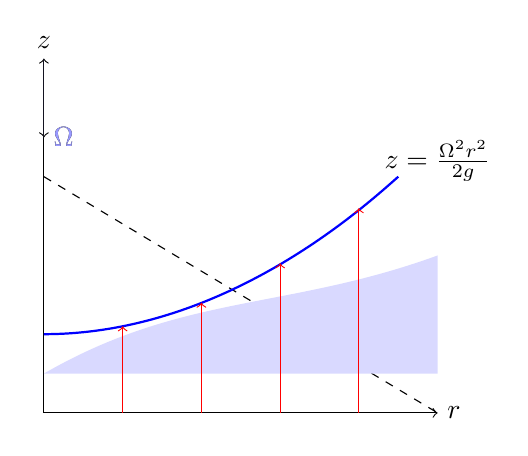
\begin{tikzpicture}[scale=1.0]
    \draw[->] (0,0) -- (0,4.5) node[above] {$z$};
    \draw[->] (0,0) -- (5,0) node[right] {$r$};
    \draw[->] (0,4.5) -- (0,3.5) node[right] {$\boldsymbol{\Omega}$};
    \draw[dashed] (0,3) -- (5,0);
    \fill[blue!15] (0,0.5) to[out=30,in=200] (5,2) -- (5,0.5) -- cycle;
    \draw[blue,thick] (0,1.0) parabola (4.5,3.0);
    \foreach \r in {1,2,3,4} {
        \draw[->,red] (\r,0) -- (\r,{1.0+0.1*\r*\r});
    }
    \node at (5,3.2) {$z=\frac{\Omega^2r^2}{2g}$};
    \fill[blue!40] (0,4.5) -- (0,3.5) node[right] {$\boldsymbol{\Omega}$};
\end{tikzpicture}
\caption{旋转容器中液体的自由面形状（旋转抛物面）}
\label{fig:rotating-vessel}
\end{figure}

该原理被应用于离心分离机：在高速旋转的容器中，由于压强分布的巨大差异，密度较大的颗粒向外侧迁移，从而实现分离。

\begin{example}
一开口圆柱形容器，直径 \(D=0.5\,\text{m}\)，初始水深 \(h_0=0.3\,\text{m}\)。容器绕中心铅直轴以 \(\Omega=100\,\text{rpm}\) 旋转。求自由面最低点的水深。

解：\(\Omega = 100\,\text{rpm} = 100\times 2\pi/60 = 10.47\,\text{rad/s}\)

旋转前后水的体积相等。抛物面下的体积：
\[
V = \pi R^2 h_{\min} + \frac{1}{2}\pi R^2 \cdot \frac{\Omega^2 R^2}{2g} = \pi R^2 h_0
\]
代入数值：\(R=0.25\,\text{m}\)，\(\frac{\Omega^2 R^2}{2g} = \frac{10.47^2\times 0.25^2}{2\times 9.81} = 0.349\,\text{m}\)
\[
h_{\min} + \frac{1}{2}\times 0.349 = 0.3 \quad \Rightarrow \quad h_{\min} = 0.126\,\text{m}
\]
\end{example}

\section{表面张力与毛细现象}

\subsection{表面张力}

液体与气体（或另一种不相溶的液体）的界面（自由表面）上存在一种使界面面积趋于最小的张力，称为表面张力（surface tension）。从分子物理学的角度看，表面张力来源于液体表面层分子受到的不平衡分子间作用力。

表面张力系数 \(\sigma\)（单位为 \(\text{N}/\text{m}\)）定义为界面上单位长度所受的张力。对于液气界面，常见液体的表面张力：

水（\(20^\circ\text{C}\)）：\(\sigma \approx 0.073\,\text{N}/\text{m}\)
水银（\(20^\circ\text{C}\)）：\(\sigma \approx 0.465\,\text{N}/\text{m}\)
乙醇（\(20^\circ\text{C}\)）：\(\sigma \approx 0.022\,\text{N}/\text{m}\)

\subsection{杨—拉普拉斯方程}

由于表面张力的存在，弯曲液面两侧存在压强差。考虑一个微小的弯曲液面元，主曲率半径分别为 \(R_1\) 和 \(R_2\)（凸面一侧的曲率为正）。杨—拉普拉斯（Young-Laplace）方程给出了跨越弯曲液面的压强跃变：

\begin{myformula}
\Delta p = p_{\text{in}} - p_{\text{out}} = \sigma\left(\frac{1}{R_1} + \frac{1}{R_2}\right)
\end{myformula}

对于球形液滴（\(R_1=R_2=R\)）：
\begin{myformula}
\Delta p = \frac{2\sigma}{R}
\end{myformula}

对于肥皂泡（有两层液面）：
\begin{myformula}
\Delta p = \frac{4\sigma}{R}
\end{myformula}

由杨—拉普拉斯方程可知，液滴越小，内外压强差越大。这解释了为什么小气泡的平衡压强更高（小气泡在液体中更难以稳定存在，因为气体趋向于从高压区扩散到低压区）。

\subsection{接触角与毛细现象}

当液体与固体壁面接触时，在三相交界处，液气界面与固体壁面之间的夹角称为接触角（contact angle）\(\theta_c\)。接触角由界面张力的平衡（杨氏方程）决定：

\begin{myformula}
\sigma_{sg} = \sigma_{sl} + \sigma_{lg} \cos\theta_c
\end{myformula}

其中 \(\sigma_{sg}\)、\(\sigma_{sl}\)、\(\sigma_{lg}\) 分别为固气、固液、液气界面的表面张力系数。

根据接触角的大小可判断润湿性：
\begin{itemize}
    \item \(\theta_c < 90^\circ\)：液体润湿固体表面（如水在玻璃表面），形成凹液面。
    \item \(\theta_c > 90^\circ\)：液体不润湿固体表面（如水银在玻璃表面），形成凸液面。
\end{itemize}

当细管（毛细管）插入液体中时，由于表面张力和润湿作用，管内液面将上升或下降。设毛细管半径为 \(r\)，平衡时液柱上升高度为 \(h\)（润湿情况）或下降 \(h\)（不润湿情况）：

由力平衡，表面张力的铅直分量 \(2\pi r \sigma \cos\theta_c\) 与液柱重力 \(\rho g (\pi r^2) h\) 平衡，得：

\begin{myformula}
h = \frac{2\sigma \cos\theta_c}{\rho g r}
\end{myformula}

此即毛细上升（Jurin）公式。对于水在玻璃管中，\(\theta_c \approx 0^\circ\)，\(\cos\theta_c \approx 1\)，则：
\[
h \approx \frac{2\times 0.073}{1000\times 9.81\times r} \approx \frac{1.49\times 10^{-5}}{r}\,\text{m}
\]

当 \(r = 1\,\text{mm}\) 时，\(h \approx 15\,\text{mm}\)；当 \(r = 0.1\,\text{mm}\) 时，\(h \approx 150\,\text{mm}\)。可见毛细效应在细管中非常显著。

毛细现象在自然界和工程中广泛存在：土壤中水分的上升、植物中水分的输运、灯芯的吸油作用、多孔介质中的渗流以及微型装置中的流体操控等。

\subsection{本章小结}

本章系统阐述了流体静力学的基本原理。我们从静止流体应力各向同性的特性出发，导出了流体静力学基本方程 \(\Nabla p = \rho\mathbf{g}\)。在重力场中得到了压强随深度线性分布的结论，以及帕斯卡原理。详细讨论了平面和曲面上静水总压力的计算方法，包括压力中心和压力体概念。推导了阿基米德浮力原理。研究了非惯性坐标系中（等加速运动和旋转）流体的平衡问题。最后介绍了表面张力和毛细现象的基本理论。流体静力学是工程水力学、船舶力学等领域的重要基础。

\begin{myalgorithm}{平面静水总压力和压力中心计算}
\begin{mycode}
import numpy as np

def hydrostatic_force_plane(rho, g, hc, A):
    """
    计算平面上的静水总压力
    rho: 流体密度 [kg/m^3]
    g: 重力加速度 [m/s^2]
    hc: 形心淹没深度 [m]
    A: 平面面积 [m^2]
    返回: 总压力 [N]
    """
    return rho * g * hc * A

def center_of_pressure(yc, Ixc, A):
    """
    计算压力中心位置
    yc: 形心到液面与壁面交线的距离 [m]
    Ixc: 面积对形心轴的惯性矩 [m^4]
    A: 平面面积 [m^2]
    返回: yD [m]
    """
    return yc + Ixc / (yc * A)

# 示例：矩形闸门
rho = 1000; g = 9.81
b, h = 2.0, 3.0         # 宽 x 高 [m]
h0 = 1.0                 # 上缘深度 [m]
A = b * h
hc = h0 + h/2
yc = hc  # (铅直壁面)
Ixc = b * h**3 / 12

F = hydrostatic_force_plane(rho, g, hc, A)
yD = center_of_pressure(yc, Ixc, A)

print(f"总压力 F = {F/1000:.1f} kN")
print(f"压力中心 yD = {yD:.2f} m (形心 yc = {yc:.2f} m)")
\end{mycode}
\end{myalgorithm}
